\subsection{Sprint 3}

Na Sprint 3, o foco do meu trabalho se concentrou na construção das visualizações de dados do painel administrativo, etapa essencial para que administradores pudessem efetivamente acompanhar a saúde do negócio como um todo. Implementei o gráfico de rosca (\textit{doughnut chart}) de status das empresas cadastradas, integrando-o à camada de serviços e ao \textit{schema} de dados do \textit{dashboard}, e também padronizei o comportamento dos \textit{tooltips} entre os diferentes gráficos do painel, incluindo o gráfico de reuniões por mês, garantindo uma experiência visual consistente em toda a aplicação. Ambas as contribuições foram submetidas em \textit{pull requests} próprios, revisadas e integradas à \textit{branch} de desenvolvimento ainda durante a sprint.

\begin{figure}[H]
    \centering
    \small
    \caption{Painel do administrador com as visualizações de dados implementadas}
    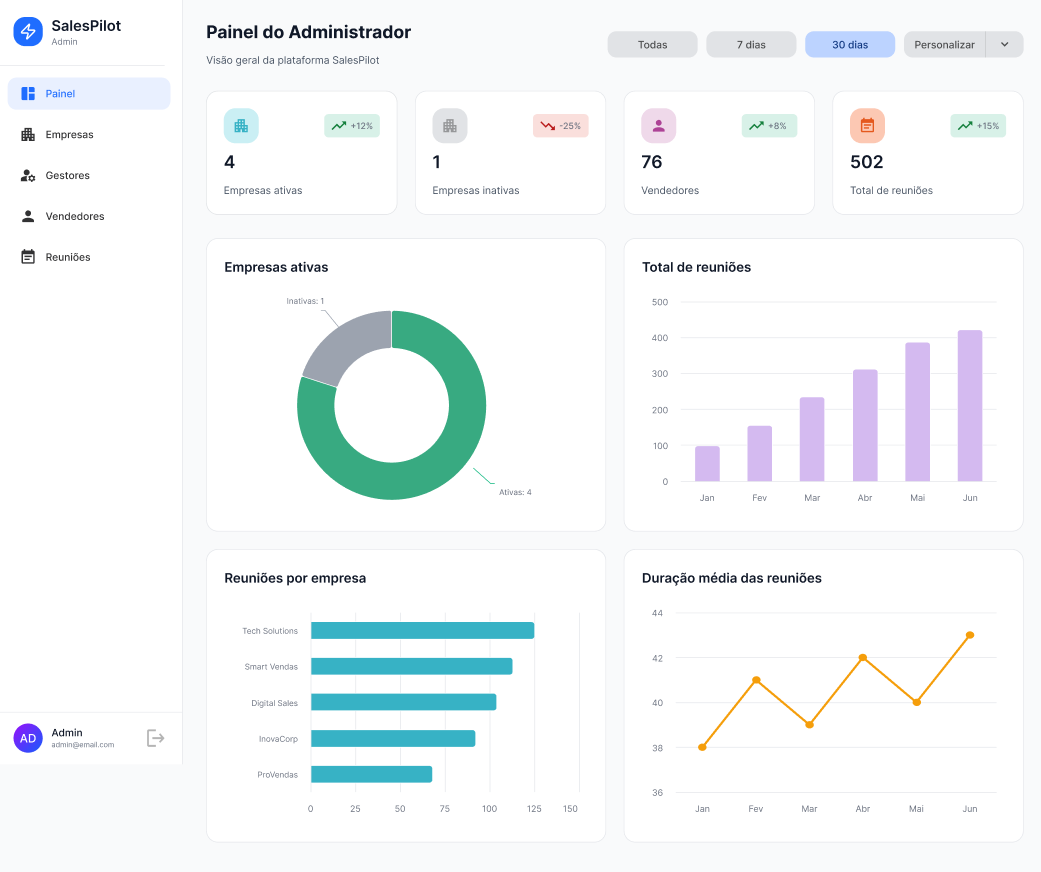
\includegraphics[width=1\linewidth]{conteudo/4 - ages III/conteudo/figures/admin_dashboard_mockup.png}\\
    \label{fig:admin-dashboard-mockup}
    \href{https://tools.ages.pucrs.br/salespilot/wiki/-/wikis/Design-Mockups}{\textit{Fonte: https://tools.ages.pucrs.br/salespilot/wiki/-/wikis/Design-Mockups}}
\end{figure}

Além do desenvolvimento próprio, dediquei uma parcela significativa do meu tempo à revisão e validação de contribuições de colegas de equipe, papel que assumi naturalmente dada minha responsabilidade pela arquitetura do frontend. Validei e fiz o \textit{merge} de \textit{pull requests} como o filtro de empresas ativas no seletor utilizado pelos formulários de cadastro e o conjunto de \textit{cards} de métricas com \textit{InsightChip} do painel do gestor, ambos desenvolvidos por colegas de equipe. Esse processo de revisão exigiu atenção redobrada para assegurar que as novas telas respeitassem os padrões de \textit{feature-based architecture} e a separação entre componentes de apresentação e de lógica definidos desde a Sprint 0, evitando que o crescimento acelerado do número de telas comprometesse a consistência do projeto.

O principal desafio da sprint foi justamente balancear o tempo entre produzir minhas próprias entregas e garantir a qualidade do que estava sendo integrado por outros membros do time. Diversos colegas atrasaram a finalização de suas \textit{tasks}, o que comprimiu o tempo disponível para uma revisão cuidadosa dos \textit{pull requests} antes da entrega, exigindo uma rodada intensa de validações em pouco tempo para que tudo fosse integrado. Como integrantes de \ac{ages} III, coube a mim e aos colegas na mesma posição corrigir boa parte das inconsistências encontradas durante essa revisão de última hora, já que não havia mais tempo disponível para devolver as correções aos autores originais. Esse acúmulo se refletiu diretamente na retrospectiva de encerramento, na qual outros colegas reclamaram da demora na revisão das PRs. Levantei nesse momento o ponto de que o problema de fundo não era a velocidade da revisão em si, mas o fato de as \textit{tasks} estarem sendo fechadas perto demais da entrega, o que não deixava tempo hábil para revisar com calma nem para que os próprios autores aplicassem eventuais ajustes solicitados.

Encerrada a Sprint 3, ficou a lição de que o papel de referência técnica em arquitetura traz consigo uma responsabilidade contínua de revisão que precisa ser planejada com a mesma seriedade que as tarefas de desenvolvimento, sob risco de se tornar um gargalo para o time, mas que essa responsabilidade só pode ser exercida com qualidade se as entregas dos colegas também respeitarem prazos que deixem espaço para a revisão. Com o painel administrativo amadurecido e seus principais gráficos entregues, o foco da equipe se direcionou para a Sprint 4, com a substituição definitiva dos dados mockados pela integração real com o backend e o avanço sobre os fluxos do gestor e do vendedor.
